\documentclass[lettersize,journal]{IEEEtran}
\usepackage{amsmath,amsfonts}
\usepackage{algorithmic}
\usepackage{algorithm}
\usepackage{array}
\usepackage[caption=false,font=normalsize,labelfont=sf,textfont=sf]{subfig}
\usepackage{textcomp}
\usepackage{stfloats}
\usepackage{url}
\usepackage{verbatim}
\usepackage{graphicx}
\usepackage{cite}
\hyphenation{op-tical net-works semi-conduc-tor IEEE-Xplore}
% updated with editorial comments 8/9/2021

\begin{document}

\title{Digital Twins: A Simulation-Based Realtime Deep Reinforcement Learning Approach for Fighting Wildfires}

\author{Jose Tupayachi,~\IEEEmembership{Grad Student,~UTK,}
        % <-this % stops a space
\thanks{This paper was produced by the IEEE Publication Technology Group. They are in Piscataway, NJ.}% <-this % stops a space
\thanks{Manuscript received April 19, 2021; revised August 16, 2021.}}

% The paper headers
\markboth{Journal of \LaTeX\ Class Files,~Vol.~14, No.~8, August~2021}%
{Shell \MakeLowercase{\textit{et al.}}: A Sample Article Using IEEEtran.cls for IEEE Journals}

\IEEEpubid{0000--0000/00\$00.00~\copyright~2021 IEEE}
% Remember, if you use this you must call \IEEEpubidadjcol in the second
% column for its text to clear the IEEEpubid mark.

\maketitle

\begin{abstract}
  This research introduces a pioneering methodology for wildfire management, employing Digital Twins in conjunction with a real-time Deep Reinforcement Learning (DRL) framework. The experimentation involves parameterized scenarios within simulated environments, with the digital twin operating in two key stages. Initially, fire stations are strategically selected based on their capacities, followed by a collaborative engagement of clustered stations in firefighting activities. The deep reinforcement model guides this collaboration, optimizing the decision-making process. An allocation approach is applied to assign firefighting entities strategically, utilizing real-time satellite imagery, a routing engine, and the fire index of each station. This ensures a coordinated and prompt response to evolving wildfire situations. In the subsequent stage, selected stations are grouped into clusters, representing independent agents, while fire events serve as the dynamic environment influencing agent actions. Agents aim to derive optimal policies in real time to minimize the impact of wildfires on the population. The holistic approach presented in this study strives to synergize resources efficiently, using real-time data, to create an adaptive and effective wildfire response system.

\end{abstract}

\begin{IEEEkeywords}
Wildfires, Deep Reinforcement Learning, Resource Allocation, Digital Twins, Realtime Decision Making, Resource Allocation.
\end{IEEEkeywords}

\section{Introduction}\label{introduction}
\IEEEPARstart{W}{ildfires} are one of the most expensive and deadly natural catastrophes in the world, particularly in the western United States. 
In 2018, a catastrophic wildfire known as the Camp Fire was recorded as one of the worst wildfires in the history of California. 
Yet these catastrophic fires are expected increase by the year 2050 [1] if preventive actions are not taken nor improvement of response services are studied. These fire events are responsible of large-scale evacuation, homes being set on fire, 
infrastructure being destroyed, millions of hectares of forest resources damaged, and most critically, human lives being in danger.
% BACKGROUND
Wildfires impact populations differently communities marked by challenges—financial limitations, cultural and institutional obstacles, restricted mobility, and compromised physical health. 
Consequently, these communities stand at a heightened risk of bearing a disproportionate burden when confronted with the catastrophic effects of wildfires. 
Literature, extends that preventive measures are demeed effective are recommended under current
research shows where wildfire mitigation can be highly cost effective [3] . Although reducing hazards activities should be priorotized like as controlling wildland fuels and constructing houses and other structures to wildfire resistant requirements. 
This is a significant and long-overdue shift from long-standing wildfire tactics that have virtually entirely focused on managing fire in wildlands.
Federal reports such as "On Fire: The Report of the Wildland Fire Mitigation and Management Commission" elaborates a set of guidelines for wild fire control and prevention.
% Tech
Fire detection and monitoring technologies have evidenced an rapid increase such as ground sensors, unmaned aerial vehicle, and satellite imagery, among others.
Current systems have the following drawbacks which include delayed fire detection due to missing minor fires in the early stages, 
% Past events
This enables community leaders to pinpoint locations where older housing may require retrofitting to enhance resistance against wildfires and customize outreach initiatives to engage nonresident landowners effectively.
The relevance lies in understanding wildfire risk can assist communities in prioritizing preventative and mitigation efforts in order to target the most vulnerable individuals.
Initiatives and data based tools like those developed for the USDA Forest Service if a community is directly threatened by wildfire from adjacent combustible vegetation or indirectly threatened by embers.
% Resource allocation and fire station locaiton!
Wildfires are considered complex scenario when it comes to simulation and proper rource ahndling due to that these tend ti vary 
% hurdles and motivation
This research is motivated on the baisis of the complexity of resource allocation. As Wildfire containment involves the allocation of various resources, including firefighting personnel, equipment, and supplies. High complexity due to factors such as the dynamic nature of wildfires, varying terrain, and resource constraints
This poses a rich environment for technologies paired with simulation based platforms such as deep reinformcement learning approaches to tackle effectively the decision making process in high complexity scenarios. 
Research on simulators utilizing deep reinforcement learning for wildfire detection has primarily focused on firefighting strategies with limited emphasis on resource allocation and decision-making, despite the significant societal benefits. In a notable study [8], a decentralized deep reinforcement learning strategy is employed for a fleet of Unmanned Aerial Vehicles (UAVs) to autonomously combat forest fires. The authors opt for a deep RL approach due to the computational challenges of exact and approximate solutions using dynamic programming. Monte Carlo simulations demonstrate the superior performance of the deep RL policy compared to a manually crafted heuristic, showcasing adaptability to varying forest sizes, UAV quantities, and model parameter variations.

In another study [7], deep reinforcement learning is applied to address complex conservation decision problems, providing a conceptual and technical introduction along with annotated code. The study showcases the effectiveness of deep RL in solving sequential decision-making challenges related to fisheries management and ecological tipping points.
In our approach, parameterized experiments unfold across simulated scenarios using a digital twin. The twin operates in two stages: firstly, selecting fire stations based on their capacity, and then, clustered stations collaboratively engage in firefighting guided by the optimal policy determined by the deep reinforcement model. An allocation approach strategically assigns firefighting entities to neighboring areas, leveraging real-time data from satellite imaging and a routing engine for a coordinated and prompt response.
Subsequently, the objective is to group selected stations into clusters and fire events, treating firefighting clusters as independent agents and fire events as dynamic environments influencing agent actions. Agents seek the optimal policy to minimize wildfire impact on the population. This holistic approach aims to synergize real-time data-driven resources into an effective and adaptive response system. The primary contributions of our work lie in these innovative approaches to resource allocation, decision-making, and firefighting strategy within the context of wildfire management.


% Research in the use of simulators that base policies in deep reinformcement learning for wildfire detection has been covered
% with scarce enphasis in resource allocation and decision making, although paramountly benefits stand for society. 
% In [8] authors Employ a decentralized deep reinforcement learning (RL) strategy for a group of Unmanned Aerial Vehicles (UAVs) to autonomously address forest fires. Due to the computational intractability of exact and approximate solutions using dynamic programming without agents, the paper opts for a deep RL approach. In this approach, each UAV develops a policy based on local information. Monte Carlo simulations illustrate that the deep RL policy outperforms a manually crafted heuristic and adapts well to various forest sizes, different UAV quantities, and variations in model parameters.
% In [7] writers explore the application of deep reinforcement learning (RL) in addressing complex conservation decision problems, 
% presenting a conceptual and technical introduction along with annotated code for researchers' adoption. Focusing on dynamic and uncertain environments, RL designs agents that interact with the surroundings, and deep RL integrates deep neural networks into these agents. The study demonstrates the effectiveness of deep RL in solving sequential decision-making challenges related to fisheries management and ecological tipping points.
% Our approach will emplot parameterized experiments will unfold across a series of simulated scenarios. The digital twin operates in two stages: firstly, selecting fire stations based on their capacity, and then, the clustered stations collaboratively engage in firefighting, guided by the optimal policy determined by the deep reinforcement model. An allocation approach is employed to strategically assign firefighting entities to neighboring areas, leveraging resources indicated by the fire index of each station. This process harnesses real-time data derived from satellite imaging and a routing engine, facilitating a coordinated and prompt response.
% Following the resolution of the initial stage, our objective is to group the selected stations into clusters and fire events. Here, fire fighting clusters assume the role of independent agents, while fire events represent the dynamic environment influencing agent actions. Agents seek the optimal policy to minimize the impact of wildfires on the population. This holistic approach aims to synergize resources, driven by real-time data, into an effective and adaptive response system. The primary contributions of our work can be outlined as follows:

\begin{itemize}
    \item We introduce a digital twin framework for wildfire management with parameterized experiments to strategically allocate firefighting entities to neighboring areas based on a proposed fire station index.

    \item Utilize deep reinforcement learning to determine an optimal policy for clustered fire stations in firefighting scenarios by seeking optimal policies to minimize the impact of wildfires on the population

    \item Incorporation of real-time data from satellite imaging and a routing engine for enhanced decision-making.
    
    \item Development of a holistic and adaptive response system, integrating deep reinforcement learning for effective wildfire management.
    


    % \item Determine a minimum data ratio threshold necessary for federated learning to be a viable and effective strategy.

    
\end{itemize}


The structure of this article is as follows: Section \ref{introduction} provides an overview of the novel contribution. Section \ref{Architecture and Information Collection} introduces the necessary environment to develop the digital twin system. We introduce the problem in section \ref{Problem Description}. Under Section \ref{Methodology} the main aim of this article is expanded and the three methodological points are explored. Section \ref{Experimentation} presents the proposed parameterized scenarios. This is followed by an analysis of the policy optimization process and the results obtained, that validate the effectiveness of the presented methods. Finally the conclusion and further discussion explores potential directions for future research. The developed code is freely accessible to the public at \url{https://github.com/josetup123/Advanced_Simulation_Paper}

\section{Architecture and Information Collection}\label{Architecture and Information Collection}
  

\begin{figure*}
  \centering
  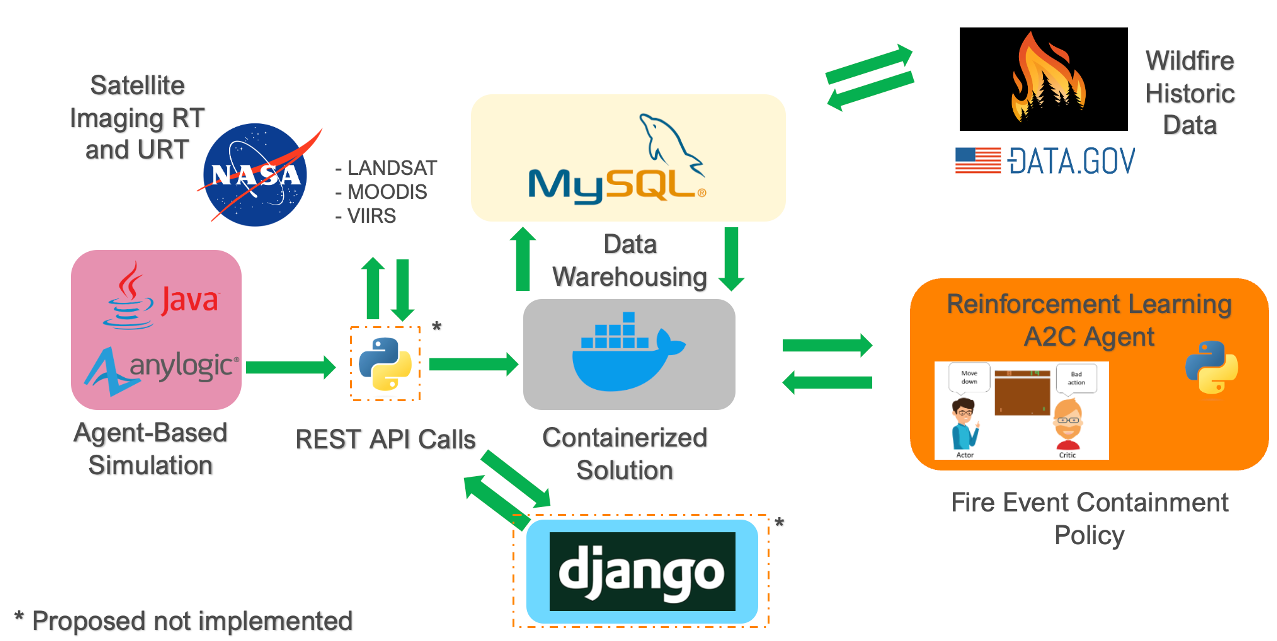
\includegraphics[height=6cm,width=12cm]{figs/Arch.png}
  \caption{
    System Architecture: The illustration depicts the fundamental components of this digital twin. Initially, satellite imaging is employed from three sources—Landsat, MODIS, and VIIRS. Each dataset is standardized, offering a confidence level for the likelihood of a fire event at each represented heat point in the future. This data is presented in tabular format and forms the basis for the backend, comprising a Django-based API and a containerized MySQL platform. The API operates as a RESTful interface for socket communication and serves as an executor of operations within the inner backend. Real-time traffic information is sourced from TomTom live data, communicating with the OSRM routing engine to generate a realistic cost matrix for transportation in optimizing neighboring station placement. Following optimization, the results are visualized in the AnyLogic GUI. The second stage involves a reinforcement learning-based policy aiming to select the policy that minimizes the economic impact caused by a fire event. An advantage actor-critic is utilized to train independent clusters for each agent, empowering them to decide on the necessary containment actions for fire events. }\label{fig:arch}
  
\end{figure*}

\section{Problem Description}\label{Problem Description}

\subsection{Stage 1}
Defining the most economically efficient fire response for a particular set of fires requires determining which resources should be dispatched to contain the fire at minimum cost. This constitutes an optimization problem that lends itself to Integer Programming (IP) because fire-fighting resources are indivisible units and are dispatched accordingly.


\subsection{Stage 2}

critical challenge is the limited effectiveness of traditional strategies in rapidly evolving and dynamic fire scenarios. Conventional approaches often struggle to adapt to the unpredictable nature of wildfires, leading to suboptimal resource allocation, delayed decision-making, and increased environmental impact
Additionally, the lack of real-time decision support systems hampers the ability of firefighting teams to respond swiftly and effectively
Develop an innovative solution that seamlessly integrates digital twins, simulation-based methodologies, and real-time deep reinforcement learning to address the shortcomings of existing wildfire management approaches. This solution aims to provide actionable insights, improve resource utilization, and minimize the environmental impact of firefighting operations, ultimately contributing to a more adaptive and proactive wildfire management paradigm

% \subsection{Simulation}


% For the simulation process we utilize four agents that represent: Heatpoints, these are entailed to generate the fire events and are created on the basis of  





\section{Methodology}\label{Methodology}


\subsection*{Pseudo Heuristic - Optimization Approach}\label{Pseudo Heuristic - Optimization Approach}

The proposed stages rely on the structure and firestation allocation that will follow a supply demand formulation. This creates an objective of reducing the total cost of allocating resources while maintaining allocating the necessary resources for wildfire suppression. The decision variables indicates the distribution of resources to the registered fire events, while constraints delimit the resources and the available limitations for the containment attempts to be effective.\\



% \textbf{Sets:}
% \begin{align}
%     & \text{Suppliers: } S = \{S_1, S_2, S_3\} \quad \text{(Set of suppliers)} \\
%     & \text{Demand Points: } D = \{D_1, D_2, D_3\} \quad \text{(Set of demand points)}
% \end{align}

% \textbf{Parameters:}
% \begin{align}
%     & \text{Supply Capacities: } S_1 = 100, S_2 = 150, S_3 = 200 \\
%     & \text{Demand: } D_1 = 80, D_2 = 120, D_3 = 150 \\
% \end{align}

\textbf{Decision Variables:}
\begin{align}
    & x_{ij} \quad \text{(Resources transported from fire station $i$ to fire event $j$)}
\end{align}

\textbf{Constraints:}
\begin{align}
    & \text{Supply Constraints:} \\
    & \quad \sum_{j} x_{ij} \leq S_i \quad \text{for each fire station $i$} \\
    & \text{Demand Constraints:} \\
    & \quad \sum_{i} x_{ij} = D_j \quad \text{for each fire point point $j$}
\end{align}

\textbf{Objective Function:}
\begin{equation}
    \text{Minimize } \sum_{i,j} c_{ij} \times x_{ij}
\end{equation}

where $c_{ij}$ represents the transportation cost from supplier $i$ to demand point $j$.




\begin{figure*}[!t]
  \normalsize % Adjust font size if necessary
  \begin{description}
    \item[$\theta$:] Parameters of the policy function.
    \item[$\phi$:] Parameters of the state-value function.
    \item[$\pi(a|s;\theta)$:] Policy function representing the probability of taking action $a$ in state $s$ with parameters $\theta$.
    \item[$R_t$:] Return at time $t$ (sum of discounted rewards over time).
    \item[$\gamma$:] Discount factor.
    \item[$A_t$:] Advantage function at time $t$, representing the advantage of taking action $a_t$ in state $s_t$.
    \item[$V(s;\phi)$:] State-value function with parameters $\phi$.
  \end{description}
  


  The A2C objective function is given by:


  \begin{align}
  &L(\theta, \phi) = \sum_{t=0}^{T} \left( \log \pi(a_t|s_t;\theta) \cdot A_t + \beta \cdot \text{H}(\pi(\cdot|s_t;\theta)) \right. \left. - \alpha \cdot \frac{1}{2} (V(s_t;\phi) - R_t)^2 \right)
\end{align}


  Where:

  \begin{align}
  &\text{H}(\pi(\cdot|s_t;\theta)) \text{ is the entropy regularization term,} \\
  &\beta \text{ is the entropy regularization coefficient,} \\
  &\alpha \text{ is the coefficient for the value function loss.}
  \end{align}
  \end{figure*}
% \subsection*{Advantage Actor-Critic (A2C)}

% The advantage actor-critic algorithm is a reinforcement learning technique that incorporates features of both policy gradient and value function approaches. A2C's mathematical formulation entails establishing the policy, value function, and objective function. The objective is to maximize this function with respect to the policy parameters  $\theta$ and the value function parameters  $\phi$.
% This mehtod is represented as follows:


% \begin{description}
%   \item[$\theta$:] Parameters of the policy function.
%   \item[$\phi$:] Parameters of the state-value function.
%   \item[$\pi(a|s;\theta)$:] Policy function representing the probability of taking action $a$ in state $s$ with parameters $\theta$.
%   \item[$R_t$:] Return at time $t$ (sum of discounted rewards over time).
%   \item[$\gamma$:] Discount factor.
%   \item[$A_t$:] Advantage function at time $t$, representing the advantage of taking action $a_t$ in state $s_t$.
%   \item[$V(s;\phi)$:] State-value function with parameters $\phi$.
% \end{description}
% % \begin{align}
% % &\theta \text{ : parameters of the policy function} \\
% % &\phi \text{ : parameters of the state-value function} \\
% % &\pi(a|s;\theta) \text{ : policy function representing the probability of taking action } a \text{ in state } s \text{ with parameters } \theta, \\
% % &R_t \text{ : return at time } t \text{ (sum of discounted rewards over time),} \\
% % &\gamma \text{ : discount factor,} \\
% % &A_t \text{ : advantage function at time } t \text{, representing the advantage of taking action } a_t \text{ in state } s_t, \\
% % &V(s;\phi) \text{ : state-value function with parameters } \phi.
% % \end{align}

% The A2C objective function is given by:\\
  

% \begin{multline}
% L(\theta, \phi) = \sum_{t=0}^{T} \left( \log \pi(a_t|s_t;\theta) \cdot A_t + \beta \cdot \text{H}(\pi(\cdot|s_t;\theta)) \right. \\
% \left. - \alpha \cdot \frac{1}{2} (V(s_t;\phi) - R_t)^2 \right),
% \end{multline}
% where:
% \begin{align}
% &\text{H}(\pi(\cdot|s_t;\theta)) \text{ is the entropy regularization term,} \\
% &\beta \text{ is the entropy regularization coefficient,} \\
% &\alpha \text{ is the coefficient for the value function loss.}
% \end{align}




\section{Experimentation}\label{Experimentation}


\subsection{Data Sources}
The system's information architecture is enriched through the judicious integration of diverse datasets, notably leveraging FIRMS (Fire Information for Resource Management System). This repository provides real-time and pertinent information on active fires, affording the system a dynamic understanding of ongoing fire events. Complementing this, the incorporation of data from Open Fire Stations enhances the spatial awareness of existing fire station locations, thereby facilitating the optimization of neighboring station placements. Furthermore, the system draws insights from original sources, notably the United States Forest Service, establishing a foundation rooted in authoritative forestry data. This comprehensive amalgamation of information from FIRMS, Open Fire Stations, and original sources contributes to the system's scholarly rigor, ensuring a nuanced understanding of the multifaceted variables inherent in fire event management and response.
The system enhances its data foundation through integration with Data.gov, a reputable source providing diverse datasets. By incorporating historical fire event registries from Data.gov, the system gains valuable insights into past incidents, enabling a nuanced analysis of patterns and trends for more informed decision-making in fire event management.

\subsection{Neighboring Station}


The determination of neighboring fire stations is derived through the following formulation, structured around a supply-demand schema. Its objective is to ascertain the optimal number of fire stations capable of responding to a fire event based on a designated index referred to as the fire\_index. This index integrates various factors obtained from independent data sources, which have been precomputed for experimental accuracy. The formulation details are provided in the subsequent lines:



% \begin{figure*}[!t]

% \textbf{Sets:}

% \begin{description}
%   \item[$S$:] Suppliers
%   \item[$D_{\text{mean}}:$] Locations (mean demand)
%   \item[$D_{\text{stddev}}:$] Standard deviations for demand
%   \item[\texttt{combined\_param}:] Cost matrix
% \end{description}

% \textbf{Parameters:}
% \begin{description}
%   \item[\texttt{num\_suppliers}:] Number of suppliers
%   \item[\texttt{num\_demand\_points}:] Number of demand points
% \end{description}

% \textbf{Constraints:}
% \begin{description}
%   \item[Supply Constraints:] $\sum_{j} x[i, j] \leq S[i]$ for each supplier $i$
%   \item[Demand Constraints:] $\sum_{i} x[i, j] = D[j]$ for each demand point $j$
% \end{description}

% \textbf{Objective Function:}
% \begin{equation}
%     \text{Minimize } \sum_{i,j} \text{combined\_param}[i][j] \times x[i, j]
% \end{equation}
% \end{figure*}




\subsection{Fire Containment}\label{Fire Containment}

\begin{figure}
  \centering
  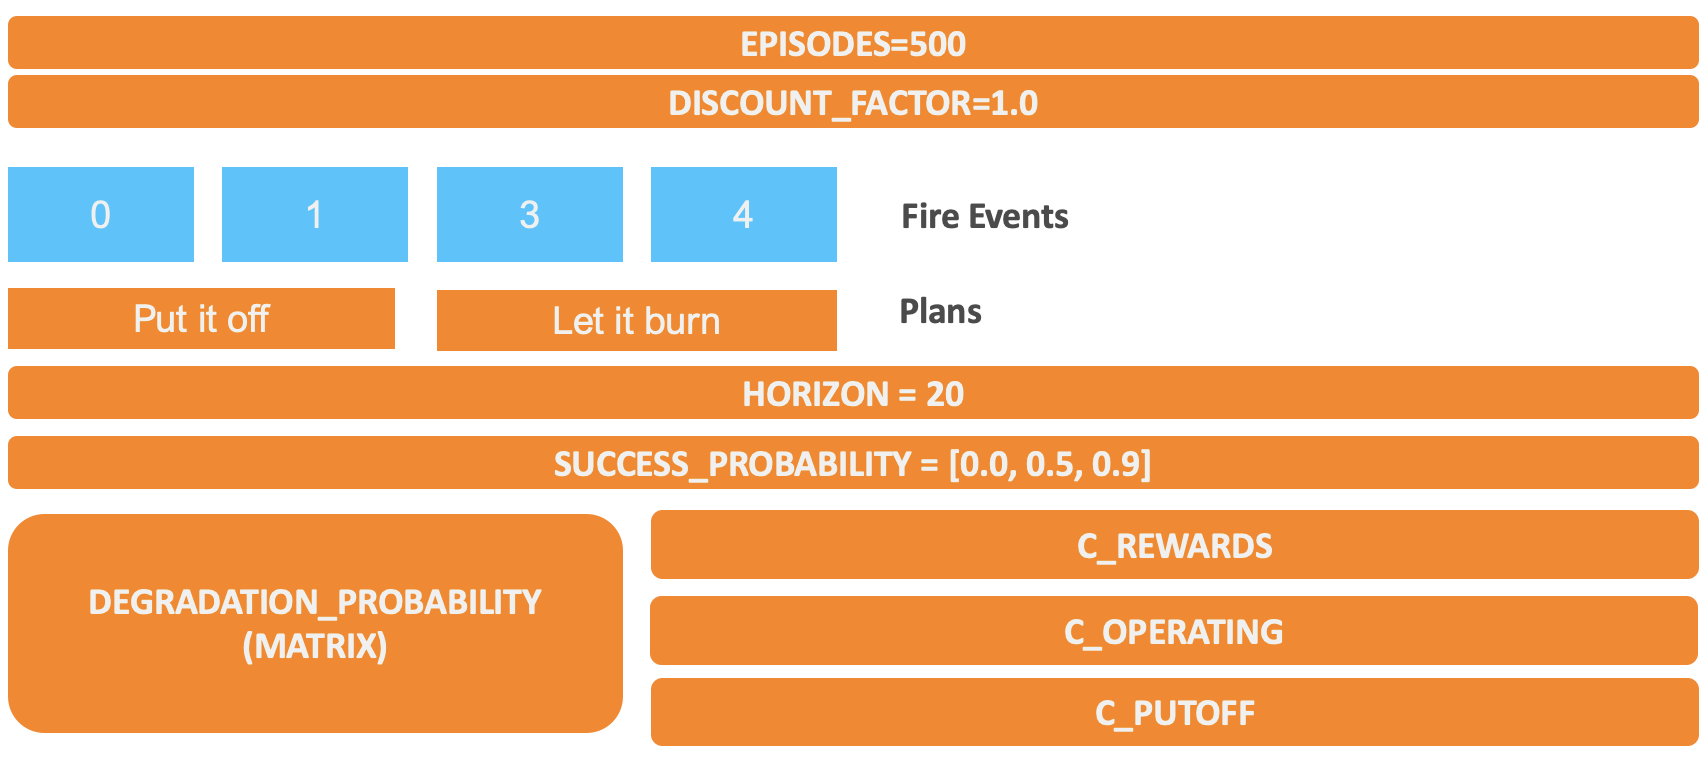
\includegraphics[height=5cm,width=8cm]{figs/parameters.png}
  \caption{Deep Reinformcement Leanring Parameters: The experimental parameters are configured as follows: \texttt{EPISODES=50000} dictates the number of agent simulations for policy improvement; \texttt{DISCOUNT\_FACTOR=1.0} emphasizes the full consideration of future rewards; \texttt{seed\_value = 42} ensures reproducibility through a set seed for the random number generator. \texttt{num\_states = Max\_FirePoints} signifies the count of environmental states, often representing diverse fire scenarios or locations. \texttt{num\_plans = 2} denotes the available action choices for the firefighter, likely relating to deciding whether to address a fire. \texttt{T = 20} defines the time horizon, indicating the number of time steps before updating policies or the simulation duration. \texttt{success\_pr = [0.0, 0.5, 0.9]} characterizes the success probability of extinguishing a fire, with values indicating varying success levels. The \texttt{degrade\_pr} matrix portrays degradation probabilities for each state, reflecting the likelihood of environmental deterioration. \texttt{C\_reward = 10} denotes the reward for fire prevention per time step, incentivizing a safe environment. \texttt{C\_Operating} encapsulates operating costs, suggesting state-dependent variations. \texttt{C\_Putoff} captures put off costs, contingent on the chosen action, likely reflecting the expenses associated with fire suppression strategies. }
\end{figure}



\begin{figure}
  \centering
  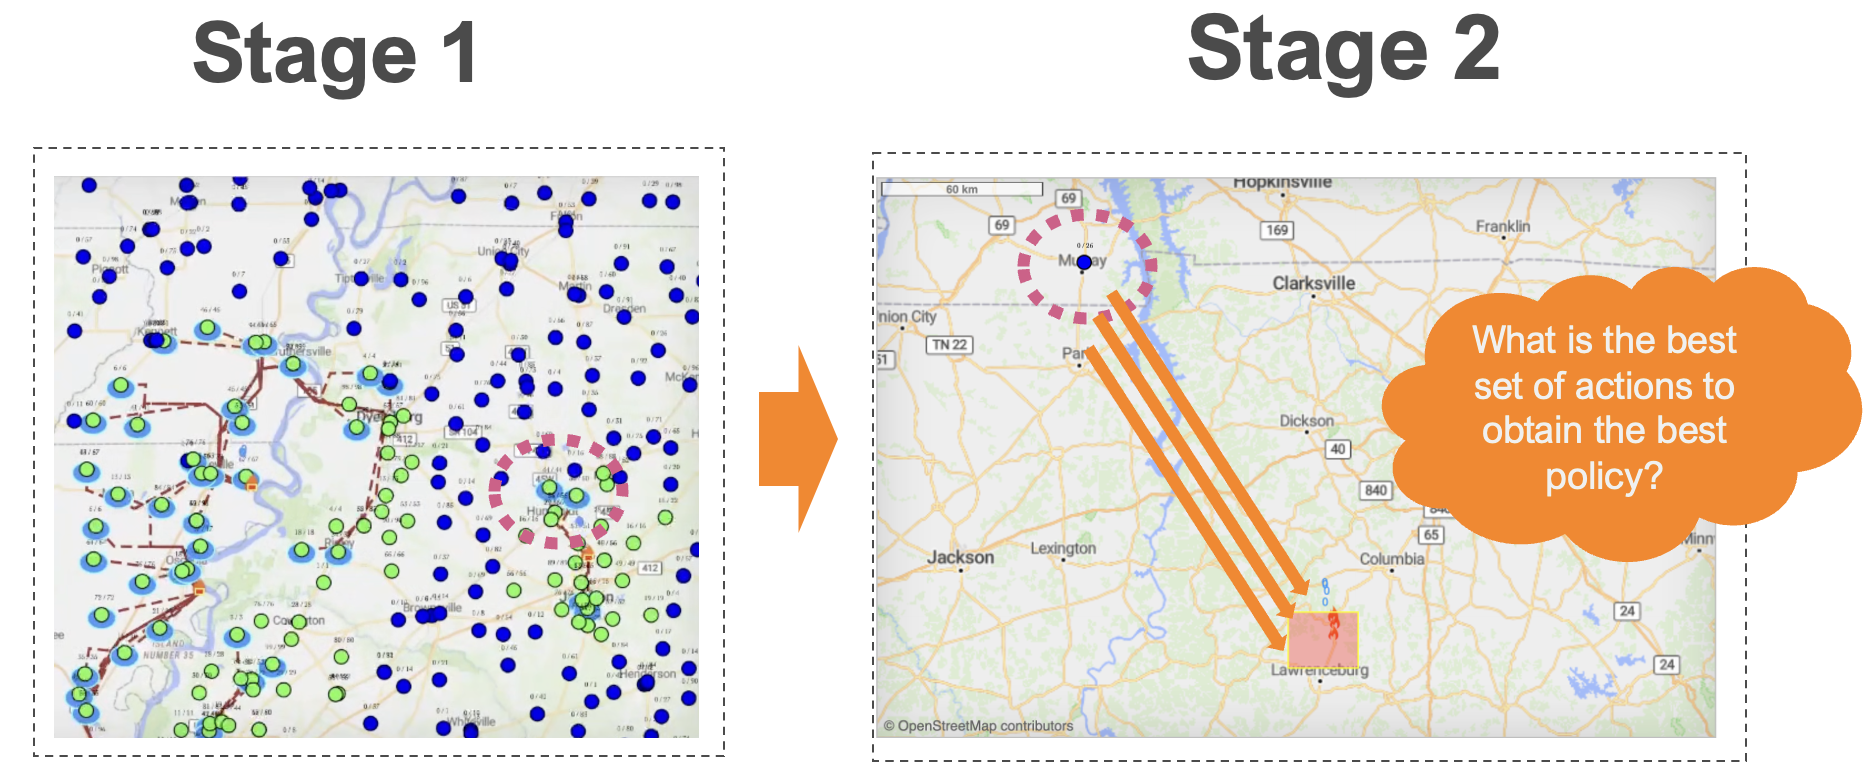
\includegraphics[height=4cm,width=9.5cm]{figs/stages.png}
  \caption{Stages Transfering: We illustrate the process of transitioning from the initial stage to the subsequent deep reinforcement learning (DRL) model in a two-stage framework. Initially, our Neighboring approach strategically allocates the requisite number of fire stations to address the prevailing number of fire events in a given area. The fire stations surrounding each fire event are then clustered, constituting Stage two. In this stage, the individual fire stations and associated resources are treated as a unified entity. The DRL approach subsequently formulates a policy, determining the optimal actions for each fire event—whether to contain, extinguish, or withhold resource allocation—at discrete time intervals, starting at $t=0$. Visualized through three arrows, these actions represent the various states the agent (comprising a cluster of fire stations and resources) can assume during the second stage. Our temporal horizon spans 20 time steps, with each step equivalent to an hour in Anylogic units, providing a comprehensive representation of the evolving dynamics.}\end{figure}


\begin{figure}
\centering
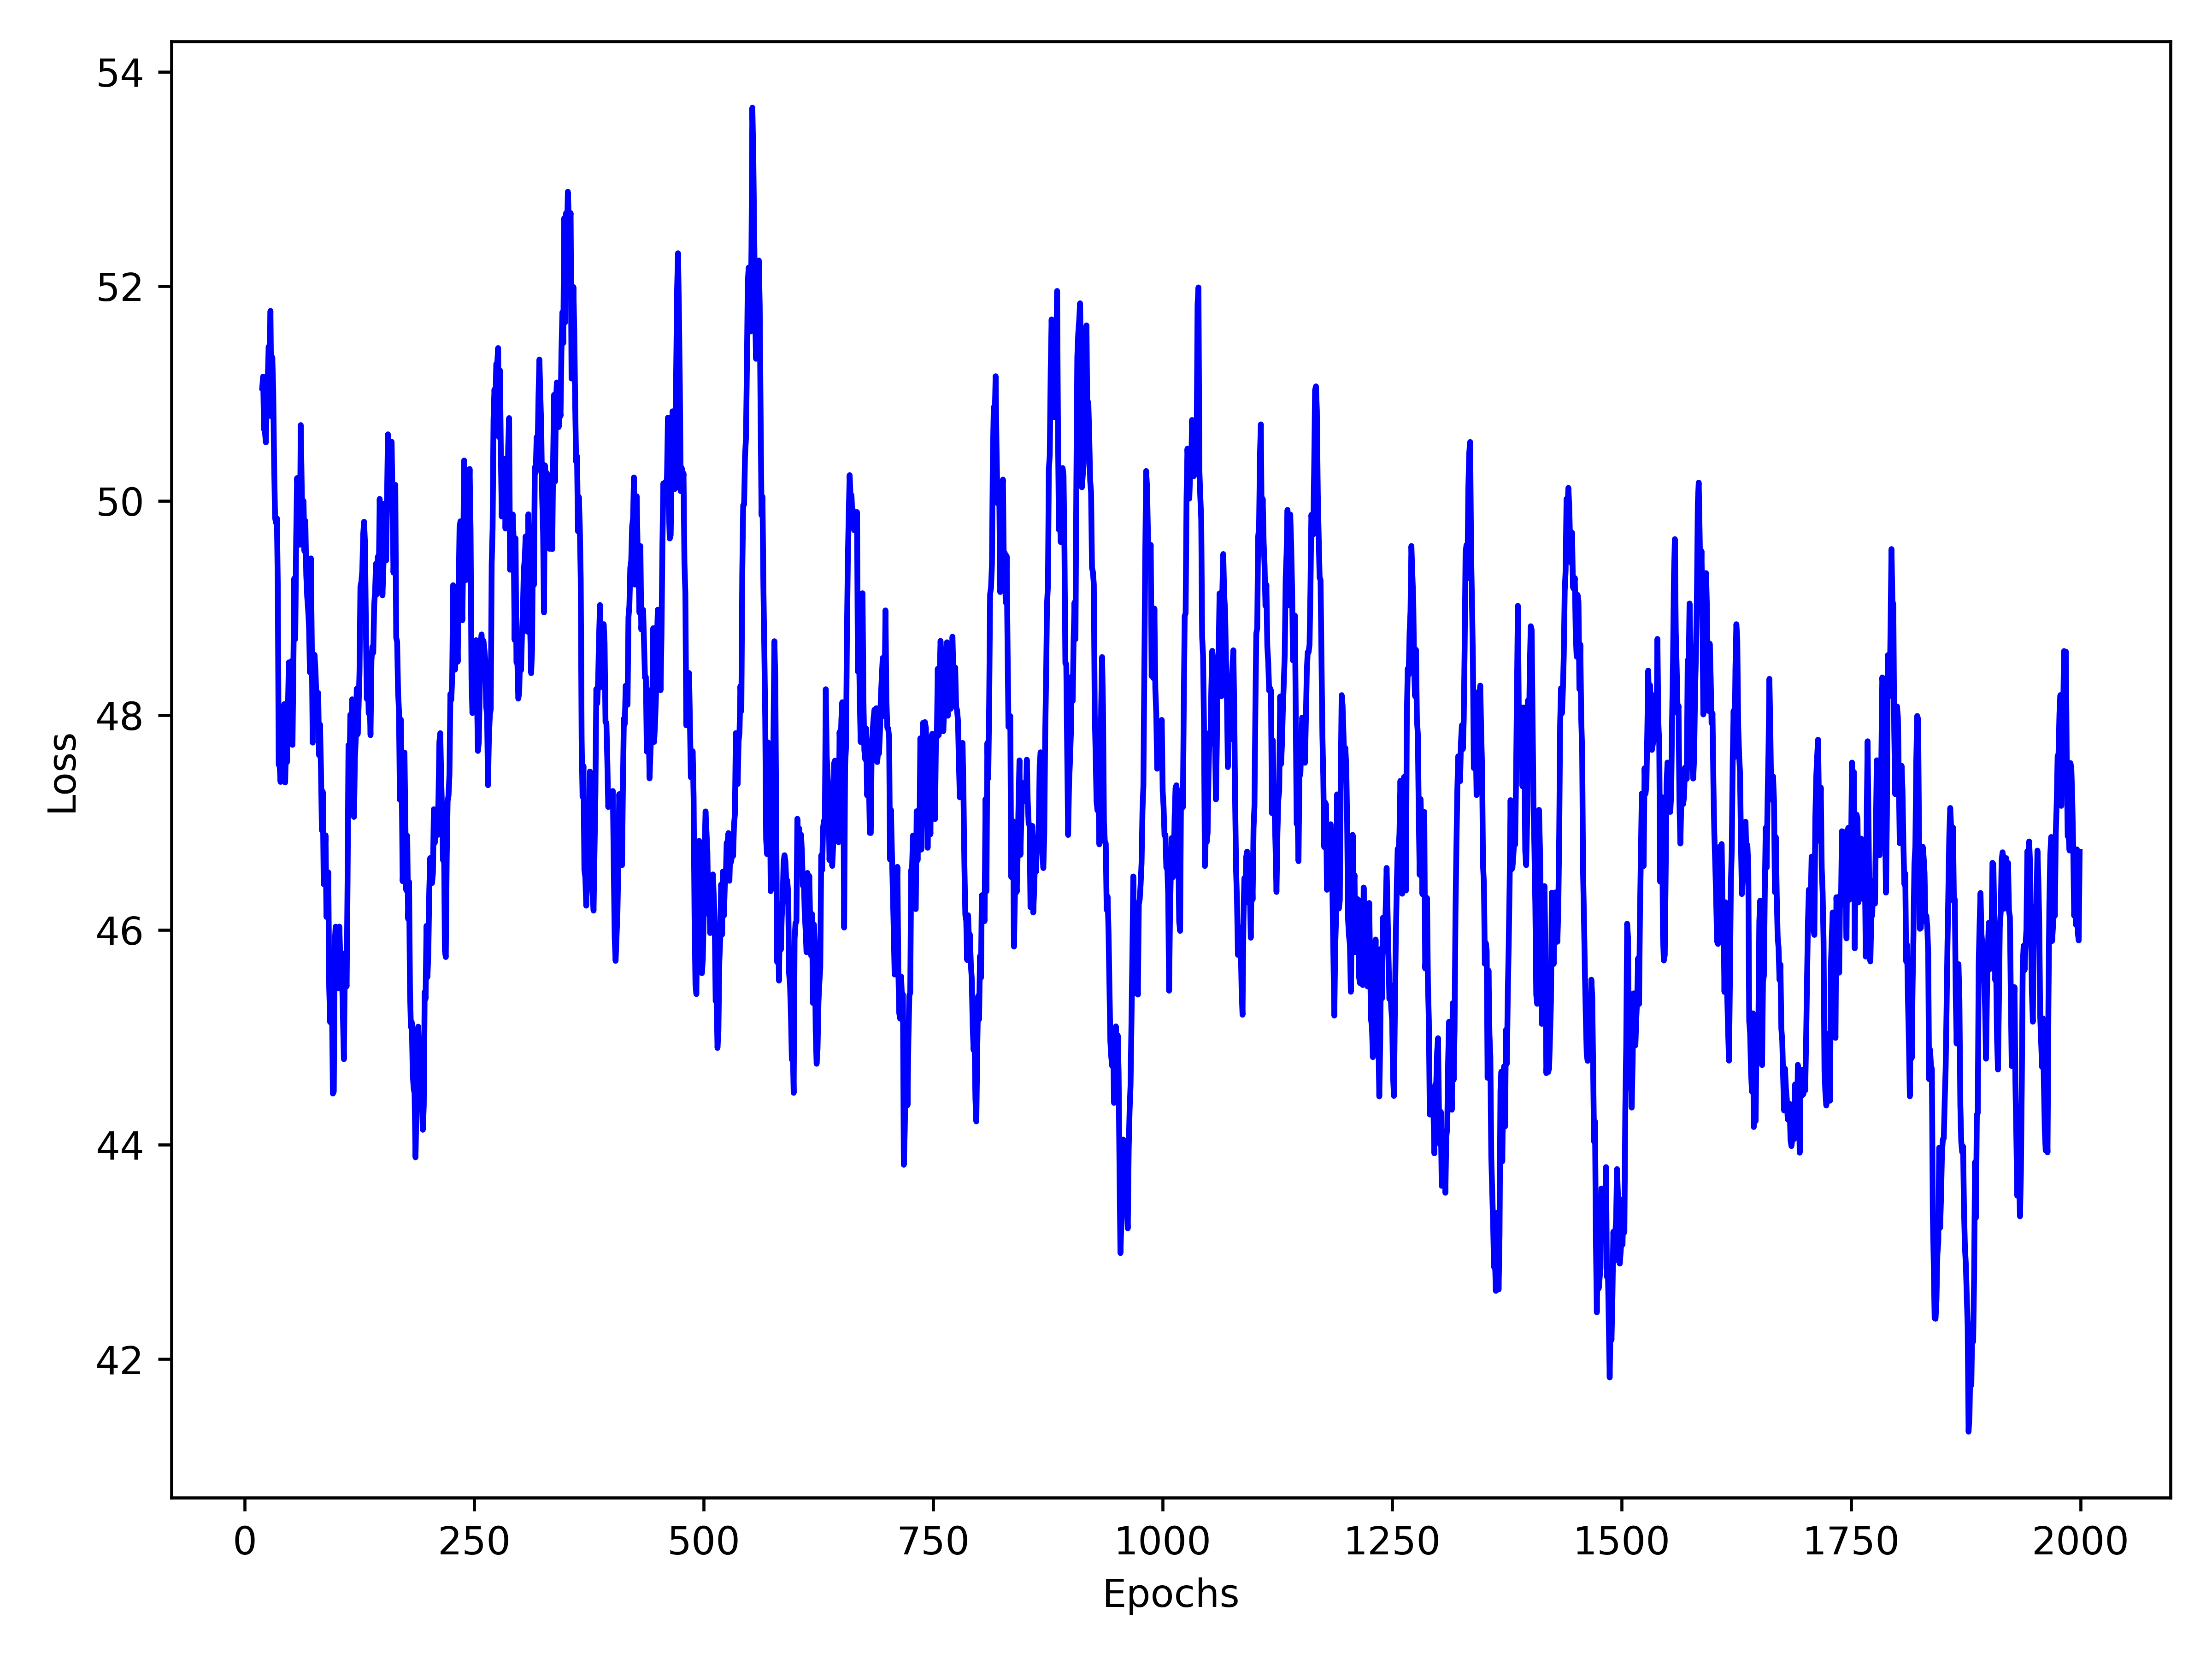
\includegraphics[height=4cm,width=8cm]{figs/manager_actor_loss.png}
\caption{Actor Loss: It indicates the cost of training the policy network. The actor loss leads policy modification to raise the likelihood of actions leading to better returns and decrease the likelihood of actions leading to lower returns. It is a component of the overall loss function, which combines actor and critic losses with the goal of maximizing the predicted cumulative reward by changing both the policy and value functions. }\end{figure}

  

\begin{figure}
\centering
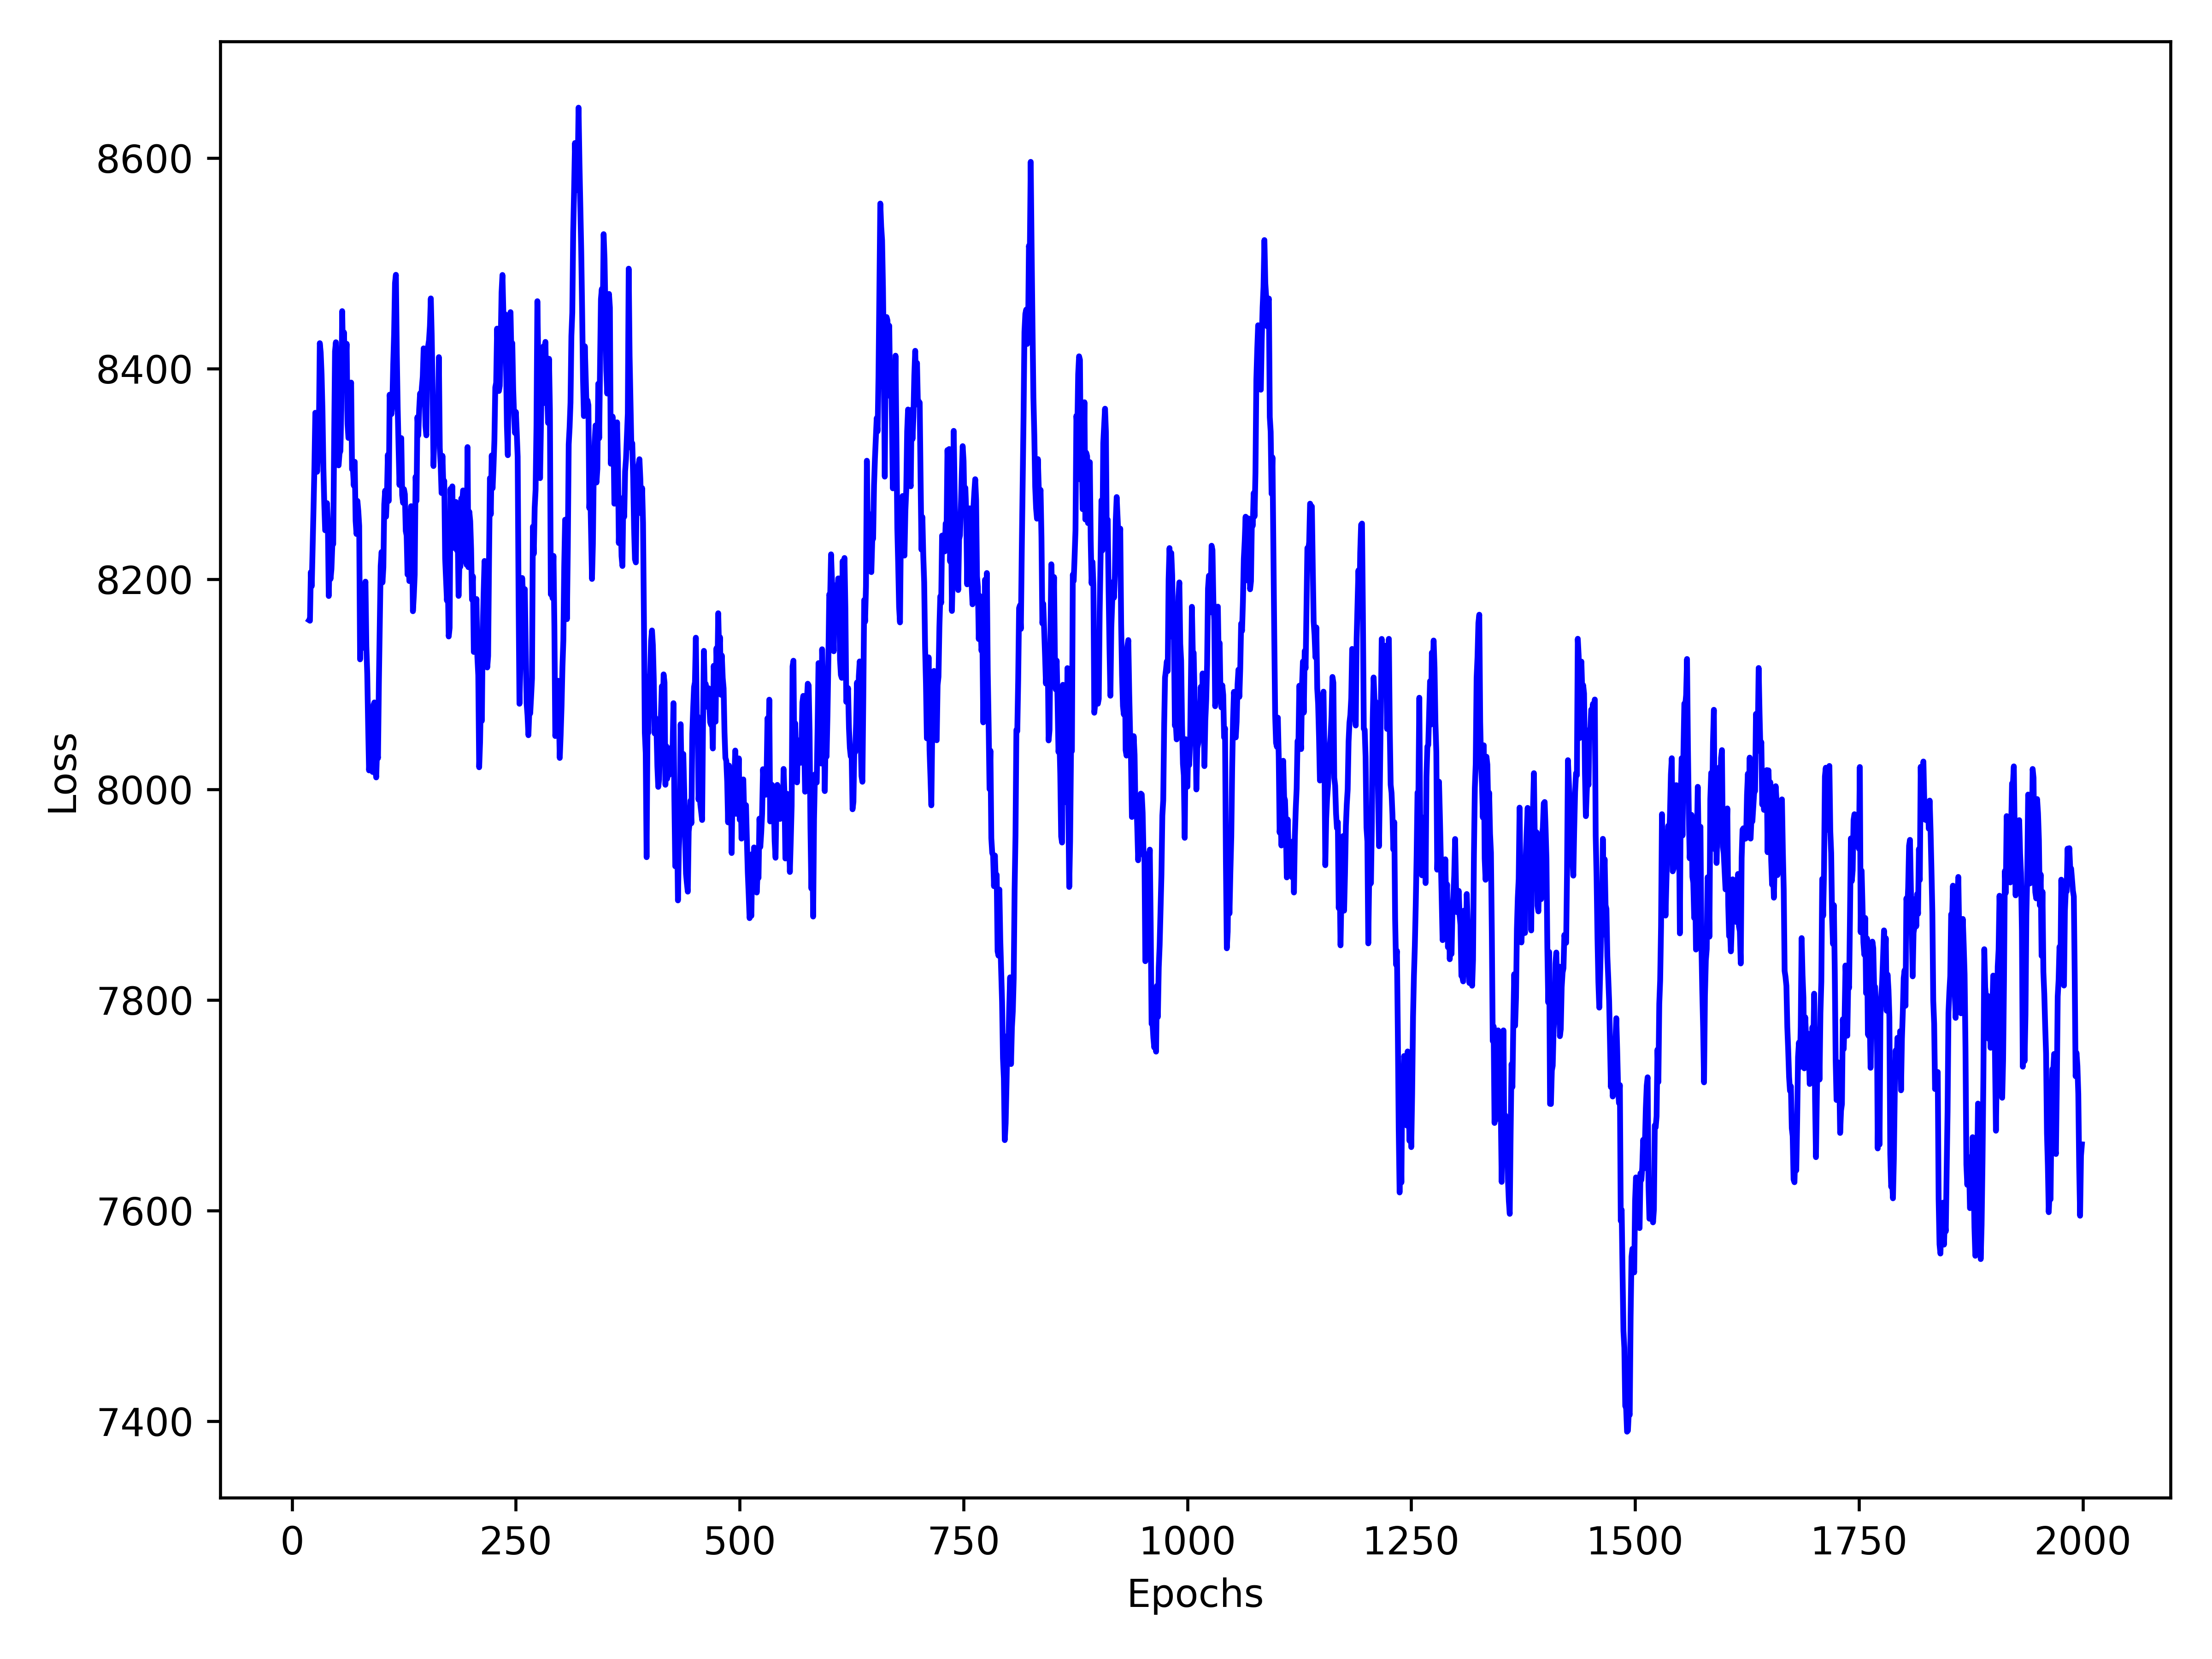
\includegraphics[height=4cm,width=8cm]{figs/manager_critic_loss.png}
\caption{Critic Loss: In Advantage Actor-Critic (A2C), the critic loss indicates the difference between the projected state value and the actual return seen during reinforcement learning training. The critic is in charge of estimating the state-value function, which calculates the predicted cumulative reward from a particular condition in A2C. The critic loss, which is frequently expressed as the mean squared error between the anticipated state value and the actual return, is a measure of how well the critic's predictions match the genuine rewards received in the environment.}\end{figure}
    
    
      \begin{figure}
        \centering
        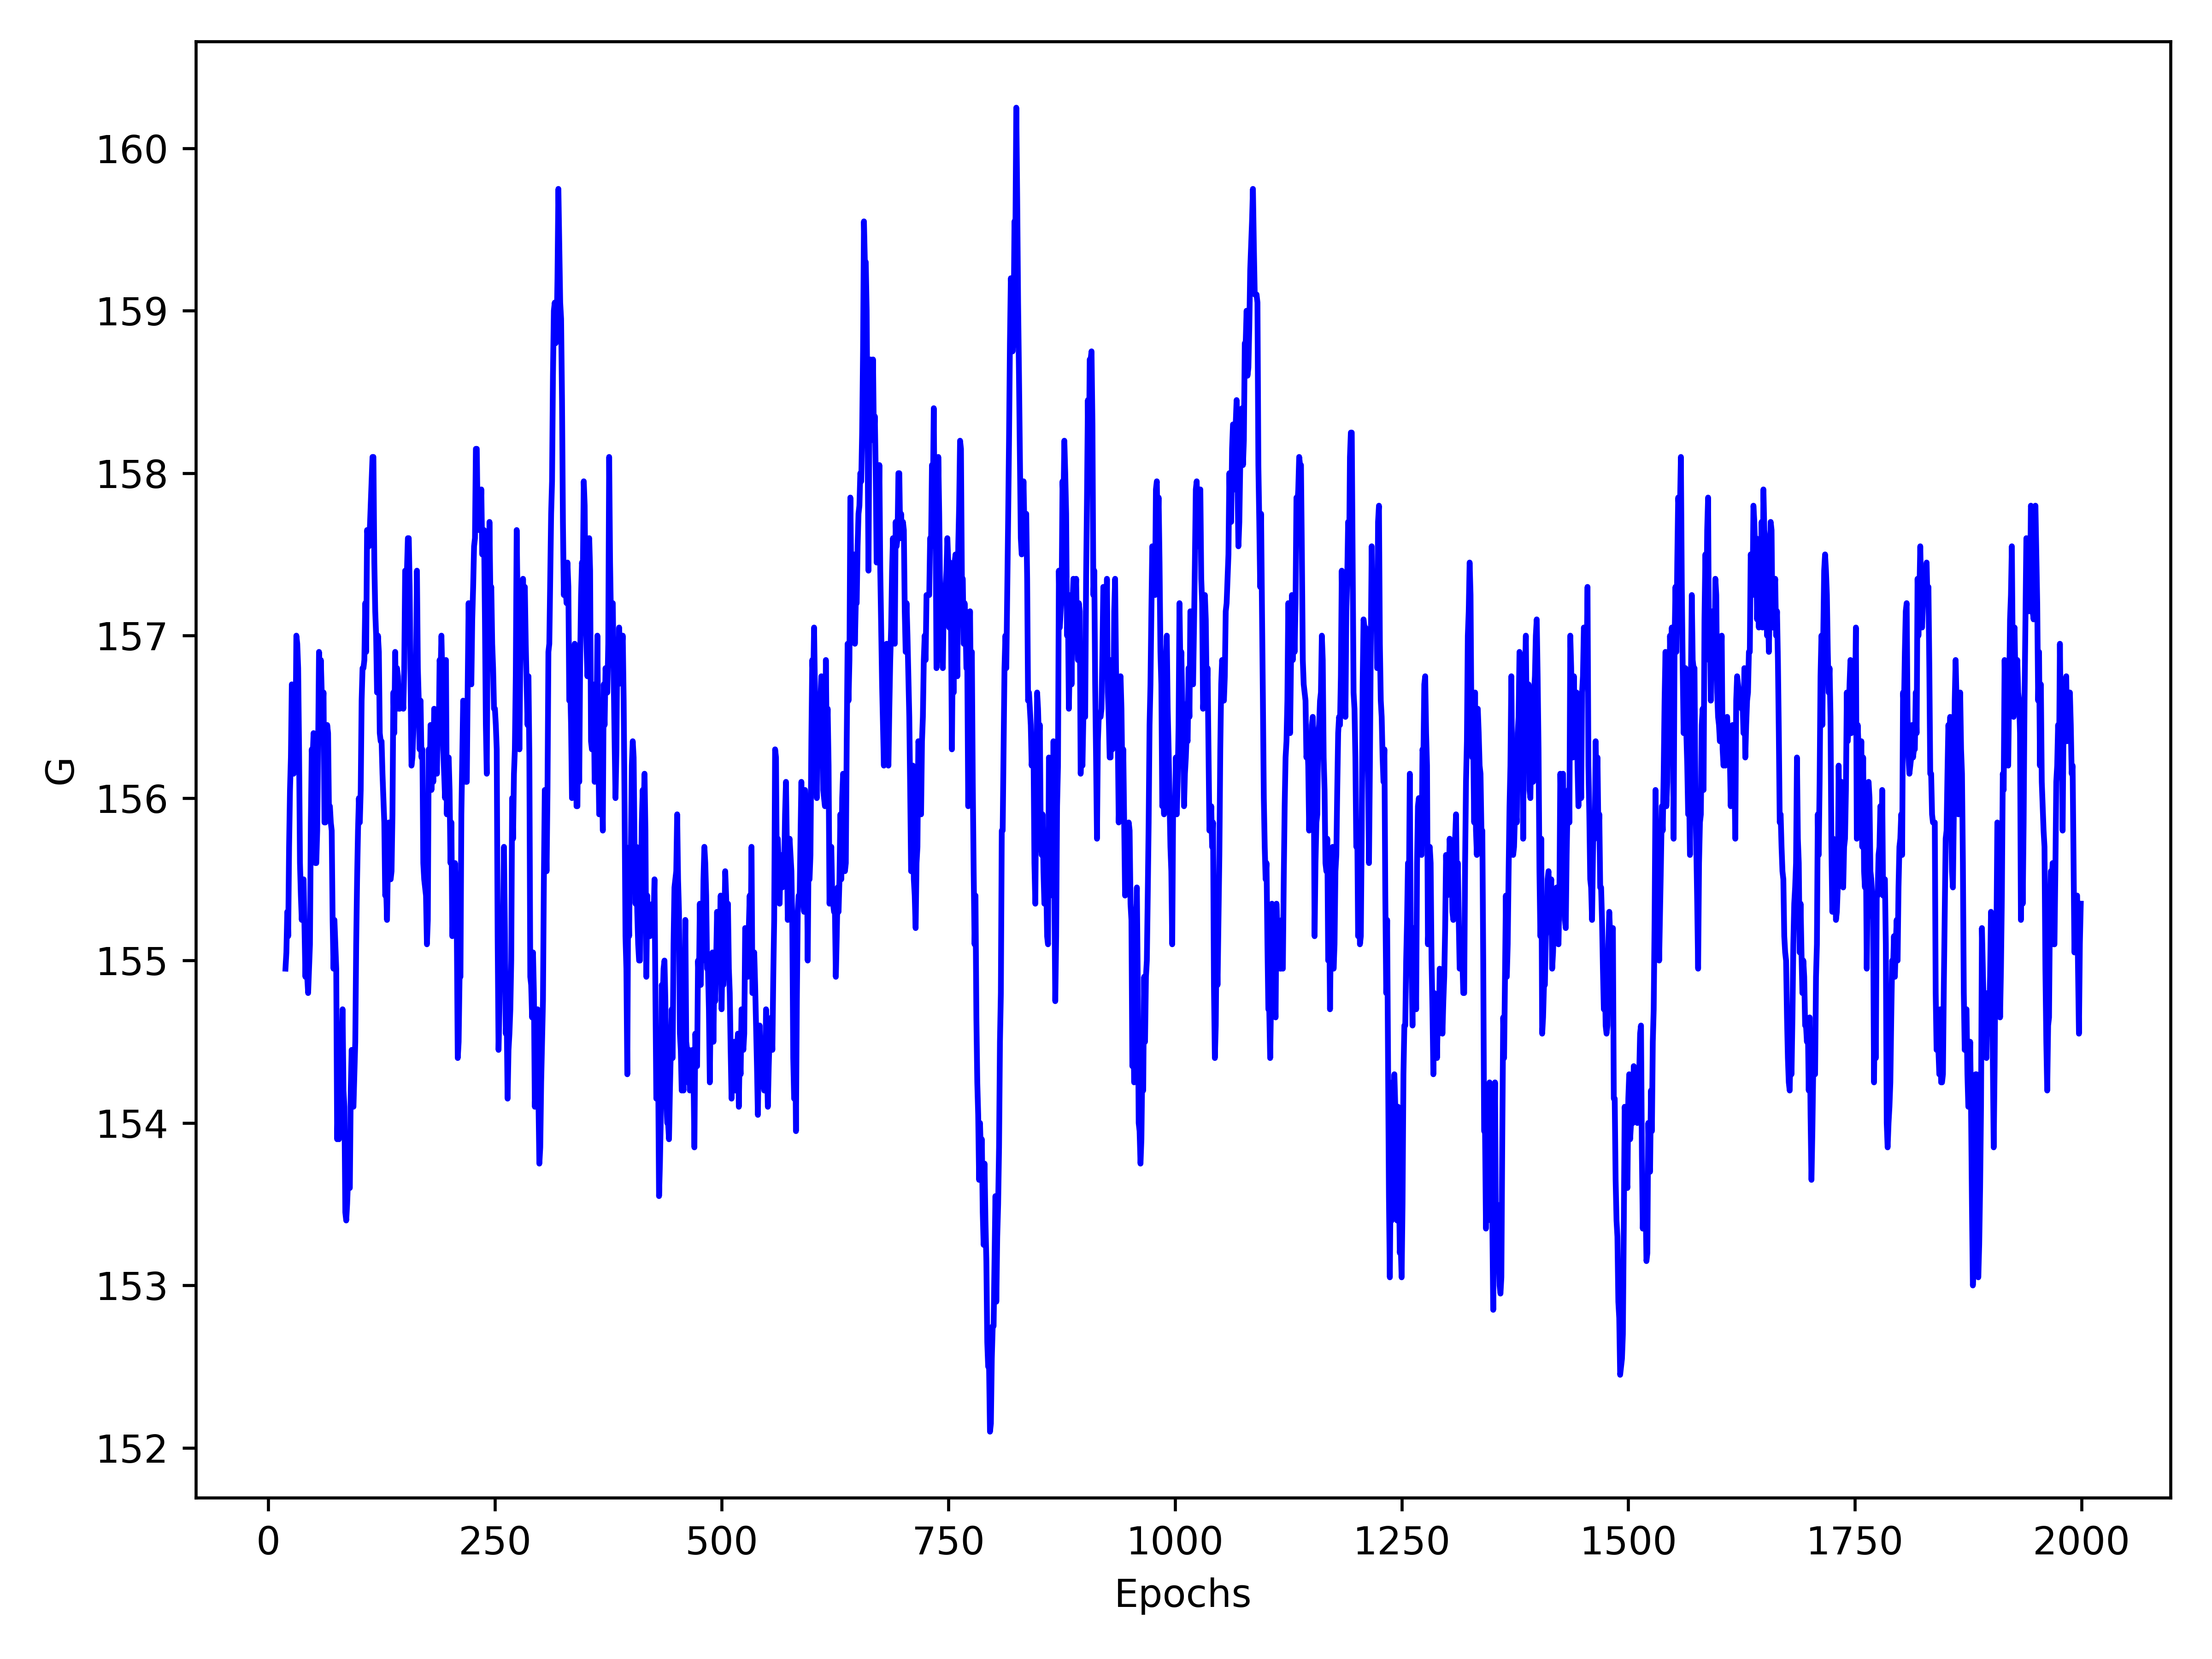
\includegraphics[height=4cm,width=8cm]{figs/manager_G.png}
        \caption{This section elucidates the profound impact of actions on the overarching policy return. A well-converged model is anticipated to showcase a discernibly smoother pattern, contrasting with the inherent noise observed during earlier stages. The graphical representation serves to illustrate the pivotal role actions play in shaping the cumulative return of the policy, offering insights into the stability and effectiveness achieved through convergence.}\end{figure}
      
      
        \begin{figure}
          \centering
          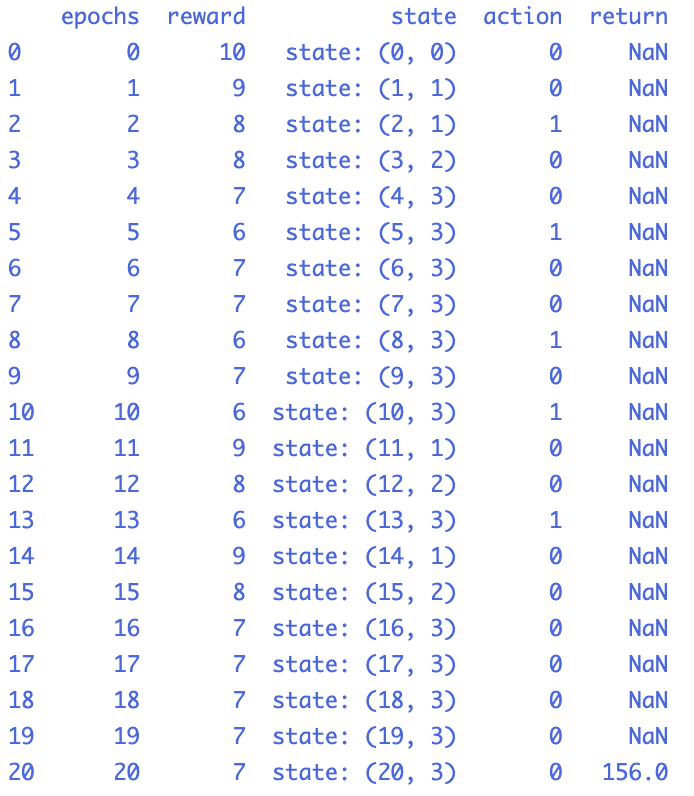
\includegraphics[height=5cm,width=5cm]{figs/4_2000.png}
          \caption{Action Schema: This comprehensive depiction provides a detailed examination of state rewards, actions, and individual states. To navigate the intricacies of the data, it is advisable to implement a state-action filter to prevent unnecessary traversal through events where fires have already been extinguished. Notably, an observable pattern emerges, highlighting the effective control measures applied to fire event 3, also denoted as state 3, which demonstrate a successful containment strategy deployed multiple times.}\end{figure}
        
        
      

          \begin{table}
            \centering
            \caption{This table represents the results of various test events conducted to assess system performance. Five distinct tests were executed, systematically increasing the number of fire events to evaluate their impact on the overall system return. Notably, our analysis focused on a carefully selected cluster of data points.
            For this specific cluster, it became evident that exceeding eight fire events would likely surpass the capacity of the fire points cluster, inevitably leading to repercussions on the population. It is crucial to emphasize that the policies implemented during these tests are still in the developmental phase. Ongoing efforts are directed towards further refinement and completion in the subsequent stages of this research.
            These findings underscore the need for cautious consideration and ongoing optimization as we progress in the development of robust policies for managing fire events.
            }
            
            
            \begin{tabular}{|c|c|c|}
              \hline
              \textbf{Test} & \textbf{Fire Events} & \textbf{Return} \\
              \hline
              1 & 4 & 156 \\
              2 & 8 & 97 \\
              3 & 80 & -961 \\
              4 & 100 & -1224 \\
              5 & 800 & -11465 \\
              \hline
              \end{tabular}
          \end{table}











% The following online groups are helpful to beginning and experienced \LaTeX\ users. A search through their archives can provide many answers to common questions.
% \begin{list}{}{}
% \item{\url{http://www.latex-community.org/}} 
% \item{\url{https://tex.stackexchange.com/} }
% \end{list}

% \section{Other Resources}
% See \cite{ref1,ref2,ref3,ref4,ref5} for resources on formatting math into text and additional help in working with \LaTeX .

% \section{Text}
% For some of the remainer of this sample we will use dummy text to fill out paragraphs rather than use live text that may violate a copyright.

% Itam, que ipiti sum dem velit la sum et dionet quatibus apitet voloritet audam, qui aliciant voloreicid quaspe volorem ut maximusandit faccum conemporerum aut ellatur, nobis arcimus.
% Fugit odi ut pliquia incitium latum que cusapere perit molupta eaquaeria quod ut optatem poreiur? Quiaerr ovitior suntiant litio bearciur?

% Onseque sequaes rectur autate minullore nusae nestiberum, sum voluptatio. Et ratem sequiam quaspername nos rem repudandae volum consequis nos eium aut as molupta tectum ulparumquam ut maximillesti consequas quas inctia cum volectinusa porrum unt eius cusaest exeritatur? Nias es enist fugit pa vollum reium essusam nist et pa aceaqui quo elibusdandis deligendus que nullaci lloreri bla que sa coreriam explacc atiumquos simolorpore, non prehendunt lam que occum\cite{ref6} si aut aut maximus eliaeruntia dia sequiamenime natem sendae ipidemp orehend uciisi omnienetus most verum, ommolendi omnimus, est, veni aut ipsa volendelist mo conserum volores estisciis recessi nveles ut poressitatur sitiis ex endi diti volum dolupta aut aut odi as eatquo cullabo remquis toreptum et des accus dolende pores sequas dolores tinust quas expel moditae ne sum quiatis nis endipie nihilis etum fugiae audi dia quiasit quibus.
% \IEEEpubidadjcol
% Ibus el et quatemo luptatque doluptaest et pe volent rem ipidusa eribus utem venimolorae dera qui acea quam etur aceruptat.
% Gias anis doluptaspic tem et aliquis alique inctiuntiur?

% Sedigent, si aligend elibuscid ut et ium volo tem eictore pellore ritatus ut ut ullatus in con con pere nos ab ium di tem aliqui od magnit repta volectur suntio. Nam isquiante doluptis essit, ut eos suntionsecto debitiur sum ea ipitiis adipit, oditiore, a dolorerempos aut harum ius, atquat.

% Rum rem ditinti sciendunti volupiciendi sequiae nonsect oreniatur, volores sition ressimil inus solut ea volum harumqui to see\eqref{deqn_ex1a} mint aut quat eos explis ad quodi debis deliqui aspel earcius.

% \begin{equation}
% \label{deqn_ex1a}
% x = \sum_{i=0}^{n} 2{i} Q.
% \end{equation}

% Alis nime volorempera perferi sitio denim repudae pre ducilit atatet volecte ssimillorae dolore, ut pel ipsa nonsequiam in re nus maiost et que dolor sunt eturita tibusanis eatent a aut et dio blaudit reptibu scipitem liquia consequodi od unto ipsae. Et enitia vel et experferum quiat harum sa net faccae dolut voloria nem. Bus ut labo. Ita eum repraer rovitia samendit aut et volupta tecupti busant omni quiae porro que nossimodic temquis anto blacita conse nis am, que ereperum eumquam quaescil imenisci quae magnimos recus ilibeaque cum etum iliate prae parumquatemo blaceaquiam quundia dit apienditem rerit re eici quaes eos sinvers pelecabo. Namendignis as exerupit aut magnim ium illabor roratecte plic tem res apiscipsam et vernat untur a deliquaest que non cus eat ea dolupiducim fugiam volum hil ius dolo eaquis sitis aut landesto quo corerest et auditaquas ditae voloribus, qui optaspis exero cusa am, ut plibus.


% \section{Some Common Elements}
% \subsection{Sections and Subsections}
% Enumeration of section headings is desirable, but not required. When numbered, please be consistent throughout the article, that is, all headings and all levels of section headings in the article should be enumerated. Primary headings are designated with Roman numerals, secondary with capital letters, tertiary with Arabic numbers; and quaternary with lowercase letters. Reference and Acknowledgment headings are unlike all other section headings in text. They are never enumerated. They are simply primary headings without labels, regardless of whether the other headings in the article are enumerated. 

% \subsection{Citations to the Bibliography}
% The coding for the citations is made with the \LaTeX\ $\backslash${\tt{cite}} command. 
% This will display as: see \cite{ref1}.

% For multiple citations code as follows: {\tt{$\backslash$cite\{ref1,ref2,ref3\}}}
%  which will produce \cite{ref1,ref2,ref3}. For reference ranges that are not consecutive code as {\tt{$\backslash$cite\{ref1,ref2,ref3,ref9\}}} which will produce  \cite{ref1,ref2,ref3,ref9}

% \subsection{Lists}
% In this section, we will consider three types of lists: simple unnumbered, numbered, and bulleted. There have been many options added to IEEEtran to enhance the creation of lists. If your lists are more complex than those shown below, please refer to the original ``IEEEtran\_HOWTO.pdf'' for additional options.\\

% \subsubsection*{\bf A plain  unnumbered list}
% \begin{list}{}{}
% \item{bare\_jrnl.tex}
% \item{bare\_conf.tex}
% \item{bare\_jrnl\_compsoc.tex}
% \item{bare\_conf\_compsoc.tex}
% \item{bare\_jrnl\_comsoc.tex}
% \end{list}

% \subsubsection*{\bf A simple numbered list}
% \begin{enumerate}
% \item{bare\_jrnl.tex}
% \item{bare\_conf.tex}
% \item{bare\_jrnl\_compsoc.tex}
% \item{bare\_conf\_compsoc.tex}
% \item{bare\_jrnl\_comsoc.tex}
% \end{enumerate}

% \subsubsection*{\bf A simple bulleted list}
% \begin{itemize}
% \item{bare\_jrnl.tex}
% \item{bare\_conf.tex}
% \item{bare\_jrnl\_compsoc.tex}
% \item{bare\_conf\_compsoc.tex}
% \item{bare\_jrnl\_comsoc.tex}
% \end{itemize}





% \subsection{Figures}
% Fig. 1 is an example of a floating figure using the graphicx package.
%  Note that $\backslash${\tt{label}} must occur AFTER (or within) $\backslash${\tt{caption}}.
%  For figures, $\backslash${\tt{caption}} should occur after the $\backslash${\tt{includegraphics}}.

% \begin{figure}[!t]
% \centering
% 
\includegraphics[width=2.5in]{fig1}
% \caption{Simulation results for the network.}
% \label{fig_1}
% \end{figure}

% Fig. 2(a) and 2(b) is an example of a double column floating figure using two subfigures.
%  (The subfig.sty package must be loaded for this to work.)
%  The subfigure $\backslash${\tt{label}} commands are set within each subfloat command,
%  and the $\backslash${\tt{label}} for the overall figure must come after $\backslash${\tt{caption}}.
%  $\backslash${\tt{hfil}} is used as a separator to get equal spacing.
%  The combined width of all the parts of the figure should do not exceed the text width or a line break will occur.
% %
% \begin{figure*}[!t]
% \centering
% \subfloat[]{
\includegraphics[width=2.5in]{fig1}%
% \label{fig_first_case}}
% \hfil
% \subfloat[]{
\includegraphics[width=2.5in]{fig1}%
% \label{fig_second_case}}
% \caption{Dae. Ad quatur autat ut porepel itemoles dolor autem fuga. Bus quia con nessunti as remo di quatus non perum que nimus. (a) Case I. (b) Case II.}
% \label{fig_sim}
% \end{figure*}

% Note that often IEEE papers with multi-part figures do not place the labels within the image itself (using the optional argument to $\backslash${\tt{subfloat}}[]), but instead will
%  reference/describe all of them (a), (b), etc., within the main caption.
%  Be aware that for subfig.sty to generate the (a), (b), etc., subfigure
%  labels, the optional argument to $\backslash${\tt{subfloat}} must be present. If a
%  subcaption is not desired, leave its contents blank,
%  e.g.,$\backslash${\tt{subfloat}}[].


 

% \section{Tables}
% Note that, for IEEE-style tables, the
%  $\backslash${\tt{caption}} command should come BEFORE the table. Table captions use title case. Articles (a, an, the), coordinating conjunctions (and, but, for, or, nor), and most short prepositions are lowercase unless they are the first or last word. Table text will default to $\backslash${\tt{footnotesize}} as
%  the IEEE normally uses this smaller font for tables.
%  The $\backslash${\tt{label}} must come after $\backslash${\tt{caption}} as always.
 
% \begin{table}[!t]
% \caption{An Example of a Table\label{tab:table1}}
% \centering
% \begin{tabular}{|c||c|}
% \hline
% One & Two\\
% \hline
% Three & Four\\
% \hline
% \end{tabular}
% \end{table}

% \section{Algorithms}
% Algorithms should be numbered and include a short title. They are set off from the text with rules above and below the title and after the last line.

% \begin{algorithm}[H]
% \caption{Weighted Tanimoto ELM.}\label{alg:alg1}
% \begin{algorithmic}
% \STATE 
% \STATE {\textsc{TRAIN}}$(\mathbf{X} \mathbf{T})$
% \STATE \hspace{0.5cm}$ \textbf{select randomly } W \subset \mathbf{X}  $
% \STATE \hspace{0.5cm}$ N_\mathbf{t} \gets | \{ i : \mathbf{t}_i = \mathbf{t} \} | $ \textbf{ for } $ \mathbf{t}= -1,+1 $
% \STATE \hspace{0.5cm}$ B_i \gets \sqrt{ \textsc{max}(N_{-1},N_{+1}) / N_{\mathbf{t}_i} } $ \textbf{ for } $ i = 1,...,N $
% \STATE \hspace{0.5cm}$ \hat{\mathbf{H}} \gets  B \cdot (\mathbf{X}^T\textbf{W})/( \mathbb{1}\mathbf{X} + \mathbb{1}\textbf{W} - \mathbf{X}^T\textbf{W} ) $
% \STATE \hspace{0.5cm}$ \beta \gets \left ( I/C + \hat{\mathbf{H}}^T\hat{\mathbf{H}} \right )^{-1}(\hat{\mathbf{H}}^T B\cdot \mathbf{T})  $
% \STATE \hspace{0.5cm}\textbf{return}  $\textbf{W},  \beta $
% \STATE 
% \STATE {\textsc{PREDICT}}$(\mathbf{X} )$
% \STATE \hspace{0.5cm}$ \mathbf{H} \gets  (\mathbf{X}^T\textbf{W} )/( \mathbb{1}\mathbf{X}  + \mathbb{1}\textbf{W}- \mathbf{X}^T\textbf{W}  ) $
% \STATE \hspace{0.5cm}\textbf{return}  $\textsc{sign}( \mathbf{H} \beta )$
% \end{algorithmic}
% \label{alg1}
% \end{algorithm}

% Que sunt eum lam eos si dic to estist, culluptium quid qui nestrum nobis reiumquiatur minimus minctem. Ro moluptat fuga. Itatquiam ut laborpo rersped exceres vollandi repudaerem. Ulparci sunt, qui doluptaquis sumquia ndestiu sapient iorepella sunti veribus. Ro moluptat fuga. Itatquiam ut laborpo rersped exceres vollandi repudaerem. 
% \section{Mathematical Typography \\ and Why It Matters}

% Typographical conventions for mathematical formulas have been developed to {\bf provide uniformity and clarity of presentation across mathematical texts}. This enables the readers of those texts to both understand the author's ideas and to grasp new concepts quickly. While software such as \LaTeX \ and MathType\textsuperscript{\textregistered} can produce aesthetically pleasing math when used properly, it is also very easy to misuse the software, potentially resulting in incorrect math display.

% IEEE aims to provide authors with the proper guidance on mathematical typesetting style and assist them in writing the best possible article. As such, IEEE has assembled a set of examples of good and bad mathematical typesetting \cite{ref1,ref2,ref3,ref4,ref5}. 

% Further examples can be found at \url{http://journals.ieeeauthorcenter.ieee.org/wp-content/uploads/sites/7/IEEE-Math-Typesetting-Guide-for-LaTeX-Users.pdf}

% \subsection{Display Equations}
% The simple display equation example shown below uses the ``equation'' environment. To number the equations, use the $\backslash${\tt{label}} macro to create an identifier for the equation. LaTeX will automatically number the equation for you.
% \begin{equation}
% \label{deqn_ex1}
% x = \sum_{i=0}^{n} 2{i} Q.
% \end{equation}

% \noindent is coded as follows:
% \begin{verbatim}
% \begin{equation}
% \label{deqn_ex1}
% x = \sum_{i=0}^{n} 2{i} Q.
% \end{equation}
% \end{verbatim}

% To reference this equation in the text use the $\backslash${\tt{ref}} macro. 
% Please see (\ref{deqn_ex1})\\
% \noindent is coded as follows:
% \begin{verbatim}
% Please see (\ref{deqn_ex1})\end{verbatim}

% \subsection{Equation Numbering}
% {\bf{Consecutive Numbering:}} Equations within an article are numbered consecutively from the beginning of the
% article to the end, i.e., (1), (2), (3), (4), (5), etc. Do not use roman numerals or section numbers for equation numbering.

% \noindent {\bf{Appendix Equations:}} The continuation of consecutively numbered equations is best in the Appendix, but numbering
%  as (A1), (A2), etc., is permissible.\\

% \noindent {\bf{Hyphens and Periods}}: Hyphens and periods should not be used in equation numbers, i.e., use (1a) rather than
% (1-a) and (2a) rather than (2.a) for subequations. This should be consistent throughout the article.

% \subsection{Multi-Line Equations and Alignment}
% Here we show several examples of multi-line equations and proper alignments.

% \noindent {\bf{A single equation that must break over multiple lines due to length with no specific alignment.}}
% \begin{multline}
% \text{The first line of this example}\\
% \text{The second line of this example}\\
% \text{The third line of this example}
% \end{multline}

% \noindent is coded as:
% \begin{verbatim}
% \begin{multline}
% \text{The first line of this example}\\
% \text{The second line of this example}\\
% \text{The third line of this example}
% \end{multline}
% \end{verbatim}

% \noindent {\bf{A single equation with multiple lines aligned at the = signs}}
% \begin{align}
% a &= c+d \\
% b &= e+f
% \end{align}
% \noindent is coded as:
% \begin{verbatim}
% \begin{align}
% a &= c+d \\
% b &= e+f
% \end{align}
% \end{verbatim}

% The {\tt{align}} environment can align on multiple  points as shown in the following example:
% \begin{align}
% x &= y & X & =Y & a &=bc\\
% x' &= y' & X' &=Y' &a' &=bz
% \end{align}
% \noindent is coded as:
% \begin{verbatim}
% \begin{align}
% x &= y & X & =Y & a &=bc\\
% x' &= y' & X' &=Y' &a' &=bz
% \end{align}
% \end{verbatim}





% \subsection{Subnumbering}
% The amsmath package provides a {\tt{subequations}} environment to facilitate subnumbering. An example:

% \begin{subequations}\label{eq:2}
% \begin{align}
% f&=g \label{eq:2A}\\
% f' &=g' \label{eq:2B}\\
% \mathcal{L}f &= \mathcal{L}g \label{eq:2c}
% \end{align}
% \end{subequations}

% \noindent is coded as:
% \begin{verbatim}
% \begin{subequations}\label{eq:2}
% \begin{align}
% f&=g \label{eq:2A}\\
% f' &=g' \label{eq:2B}\\
% \mathcal{L}f &= \mathcal{L}g \label{eq:2c}
% \end{align}
% \end{subequations}

% \end{verbatim}

% \subsection{Matrices}
% There are several useful matrix environments that can save you some keystrokes. See the example coding below and the output.

% \noindent {\bf{A simple matrix:}}
% \begin{equation}
% \begin{matrix}  0 &  1 \\ 
% 1 &  0 \end{matrix}
% \end{equation}
% is coded as:
% \begin{verbatim}
% \begin{equation}
% \begin{matrix}  0 &  1 \\ 
% 1 &  0 \end{matrix}
% \end{equation}
% \end{verbatim}

% \noindent {\bf{A matrix with parenthesis}}
% \begin{equation}
% \begin{pmatrix} 0 & -i \\
%  i &  0 \end{pmatrix}
% \end{equation}
% is coded as:
% \begin{verbatim}
% \begin{equation}
% \begin{pmatrix} 0 & -i \\
%  i &  0 \end{pmatrix}
% \end{equation}
% \end{verbatim}

% \noindent {\bf{A matrix with square brackets}}
% \begin{equation}
% \begin{bmatrix} 0 & -1 \\ 
% 1 &  0 \end{bmatrix}
% \end{equation}
% is coded as:
% \begin{verbatim}
% \begin{equation}
% \begin{bmatrix} 0 & -1 \\ 
% 1 &  0 \end{bmatrix}
% \end{equation}
% \end{verbatim}

% \noindent {\bf{A matrix with curly braces}}
% \begin{equation}
% \begin{Bmatrix} 1 &  0 \\ 
% 0 & -1 \end{Bmatrix}
% \end{equation}
% is coded as:
% \begin{verbatim}
% \begin{equation}
% \begin{Bmatrix} 1 &  0 \\ 
% 0 & -1 \end{Bmatrix}
% \end{equation}\end{verbatim}

% \noindent {\bf{A matrix with single verticals}}
% \begin{equation}
% \begin{vmatrix} a &  b \\ 
% c &  d \end{vmatrix}
% \end{equation}
% is coded as:
% \begin{verbatim}
% \begin{equation}
% \begin{vmatrix} a &  b \\ 
% c &  d \end{vmatrix}
% \end{equation}\end{verbatim}

% \noindent {\bf{A matrix with double verticals}}
% \begin{equation}
% \begin{Vmatrix} i &  0 \\ 
% 0 & -i \end{Vmatrix}
% \end{equation}
% is coded as:
% \begin{verbatim}
% \begin{equation}
% \begin{Vmatrix} i &  0 \\ 
% 0 & -i \end{Vmatrix}
% \end{equation}\end{verbatim}

% \subsection{Arrays}
% The {\tt{array}} environment allows you some options for matrix-like equations. You will have to manually key the fences, but there are other options for alignment of the columns and for setting horizontal and vertical rules. The argument to {\tt{array}} controls alignment and placement of vertical rules.

% A simple array
% \begin{equation}
% \left(
% \begin{array}{cccc}
% a+b+c & uv & x-y & 27\\
% a+b & u+v & z & 134
% \end{array}\right)
% \end{equation}
% is coded as:
% \begin{verbatim}
% \begin{equation}
% \left(
% \begin{array}{cccc}
% a+b+c & uv & x-y & 27\\
% a+b & u+v & z & 134
% \end{array} \right)
% \end{equation}
% \end{verbatim}

% A slight variation on this to better align the numbers in the last column
% \begin{equation}
% \left(
% \begin{array}{cccr}
% a+b+c & uv & x-y & 27\\
% a+b & u+v & z & 134
% \end{array}\right)
% \end{equation}
% is coded as:
% \begin{verbatim}
% \begin{equation}
% \left(
% \begin{array}{cccr}
% a+b+c & uv & x-y & 27\\
% a+b & u+v & z & 134
% \end{array} \right)
% \end{equation}
% \end{verbatim}

% An array with vertical and horizontal rules
% \begin{equation}
% \left( \begin{array}{c|c|c|r}
% a+b+c & uv & x-y & 27\\ \hline
% a+b & u+v & z & 134
% \end{array}\right)
% \end{equation}
% is coded as:
% \begin{verbatim}
% \begin{equation}
% \left(
% \begin{array}{c|c|c|r}
% a+b+c & uv & x-y & 27\\
% a+b & u+v & z & 134
% \end{array} \right)
% \end{equation}
% \end{verbatim}
% Note the argument now has the pipe "$\vert$" included to indicate the placement of the vertical rules.


% \subsection{Cases Structures}
% Many times cases can be miscoded using the wrong environment, i.e., {\tt{array}}. Using the {\tt{cases}} environment will save keystrokes (from not having to type the $\backslash${\tt{left}}$\backslash${\tt{lbrace}}) and automatically provide the correct column alignment.
% \begin{equation*}
% {z_m(t)} = \begin{cases}
% 1,&{\text{if}}\ {\beta }_m(t) \\ 
% {0,}&{\text{otherwise.}} 
% \end{cases}
% \end{equation*}
% \noindent is coded as follows:
% \begin{verbatim}
% \begin{equation*}
% {z_m(t)} = 
% \begin{cases}
% 1,&{\text{if}}\ {\beta }_m(t),\\ 
% {0,}&{\text{otherwise.}} 
% \end{cases}
% \end{equation*}
% \end{verbatim}
% \noindent Note that the ``\&'' is used to mark the tabular alignment. This is important to get  proper column alignment. Do not use $\backslash${\tt{quad}} or other fixed spaces to try and align the columns. Also, note the use of the $\backslash${\tt{text}} macro for text elements such as ``if'' and ``otherwise.''

% \subsection{Function Formatting in Equations}
% Often, there is an easy way to properly format most common functions. Use of the $\backslash$ in front of the function name will in most cases, provide the correct formatting. When this does not work, the following example provides a solution using the $\backslash${\tt{text}} macro:

% \begin{equation*} 
%   d_{R}^{KM} = \underset {d_{l}^{KM}} {\text{arg min}} \{ d_{1}^{KM},\ldots,d_{6}^{KM}\}.
% \end{equation*}

% \noindent is coded as follows:
% \begin{verbatim}
% \begin{equation*} 
%  d_{R}^{KM} = \underset {d_{l}^{KM}} 
%  {\text{arg min}} \{ d_{1}^{KM},
%  \ldots,d_{6}^{KM}\}.
% \end{equation*}
% \end{verbatim}

% \subsection{ Text Acronyms Inside Equations}
% This example shows where the acronym ``MSE" is coded using $\backslash${\tt{text\{\}}} to match how it appears in the text.

% \begin{equation*}
%  \text{MSE} = \frac {1}{n}\sum _{i=1}^{n}(Y_{i} - \hat {Y_{i}})^{2}
% \end{equation*}

% \begin{verbatim}
% \begin{equation*}
%  \text{MSE} = \frac {1}{n}\sum _{i=1}^{n}
% (Y_{i} - \hat {Y_{i}})^{2}
% \end{equation*}
% \end{verbatim}

% \section{Conclusion}
% The conclusion goes here.


% \section*{Acknowledgments}
% This should be a simple paragraph before the References to thank those individuals and institutions who have supported your work on this article.





%{\appendices
%\section*{Proof of the First Zonklar Equation}
%Appendix one text goes here.
% You can choose not to have a title for an appendix if you want by leaving the argument blank
%\section*{Proof of the Second Zonklar Equation}
%Appendix two text goes here.}

\section{Conclusion \& Further Directions}

The presented approach outlines a comprehensive digital twin framework for wildfire management that leverages various innovative technologies. The integration of parameterized experiments facilitates the strategic allocation of firefighting entities to neighboring areas, guided by a novel fire station index. The utilization of deep reinforcement learning is a key highlight, as it determines optimal policies for clustered fire stations, aiming to minimize the impact of wildfires on the population. This not only enhances the efficiency of firefighting scenarios but also demonstrates a forward-looking approach to addressing dynamic and complex challenges.

The incorporation of real-time data from satellite imaging and a routing engine further enhances decision-making capabilities, allowing for a more accurate and timely response to evolving wildfire situations. By integrating these technologies, the framework creates a holistic and adaptive response system. The emphasis on deep reinforcement learning throughout the system signifies a commitment to effective wildfire management through continuous learning and optimization. This approach represents a significant step towards leveraging cutting-edge technologies for more efficient, data-driven, and adaptive wildfire management strategies.


\section{References Section}
% You can use a bibliography generated by BibTeX as a .bbl file.
%  BibTeX documentation can be easily obtained at:
%  http://mirror.ctan.org/biblio/bibtex/contrib/doc/
%  The IEEEtran BibTeX style support page is:
%  http://www.michaelshell.org/tex/ieeetran/bibtex/
 
 % argument is your BibTeX string definitions and bibliography database(s)
%\bibliography{IEEEabrv,../bib/paper}
%
% \section{Simple References}
% You can manually copy in the resultant .bbl file and set second argument of $\backslash${\tt{begin}} to the number of references
%  (used to reserve space for the reference number labels box).



% \bibliographystyle{IEEEtran}
% \bibliography{references.bib}



% \begin{thebibliography}{1}
% \bibliographystyle{IEEEtran}

% \bibitem{ref1}
% {\it{Mathematics Into Type}}. American Mathematical Society. [Online]. Available: https://www.ams.org/arc/styleguide/mit-2.pdf

% \bibitem{ref2}
% T. W. Chaundy, P. R. Barrett and C. Batey, {\it{The Printing of Mathematics}}. London, U.K., Oxford Univ. Press, 1954.

% \bibitem{ref3}
% F. Mittelbach and M. Goossens, {\it{The \LaTeX Companion}}, 2nd ed. Boston, MA, USA: Pearson, 2004.

% \bibitem{ref4}
% G. Gr\"atzer, {\it{More Math Into LaTeX}}, New York, NY, USA: Springer, 2007.

% \bibitem{ref5}M. Letourneau and J. W. Sharp, {\it{AMS-StyleGuide-online.pdf,}} American Mathematical Society, Providence, RI, USA, [Online]. Available: http://www.ams.org/arc/styleguide/index.html

% \bibitem{ref6}
% H. Sira-Ramirez, ``On the sliding mode control of nonlinear systems,'' \textit{Syst. Control Lett.}, vol. 19, pp. 303--312, 1992.

% \bibitem{ref7}
% A. Levant, ``Exact differentiation of signals with unbounded higher derivatives,''  in \textit{Proc. 45th IEEE Conf. Decis.
% Control}, San Diego, CA, USA, 2006, pp. 5585--5590. DOI: 10.1109/CDC.2006.377165.

% \bibitem{ref8}
% M. Fliess, C. Join, and H. Sira-Ramirez, ``Non-linear estimation is easy,'' \textit{Int. J. Model., Ident. Control}, vol. 4, no. 1, pp. 12--27, 2008.

% \bibitem{ref9}
% R. Ortega, A. Astolfi, G. Bastin, and H. Rodriguez, ``Stabilization of food-chain systems using a port-controlled Hamiltonian description,'' in \textit{Proc. Amer. Control Conf.}, Chicago, IL, USA,
% 2000, pp. 2245--2249.

[1]U. Nations, “As Wildfires Increase, Integrated Strategies for Forests, Climate and Sustainability Are Ever More Urgent.” https://www.un.org/en/un-chronicle/wildfires-increase-integrated-strategies-forests-climate-and-sustainability-are-ever-0 (accessed Oct. 19, 2023).

[2]“Wilfire Risk To Communities.” https://wildfirerisk.org/ (accessed Dec. 14, 2023). 

[3]P. Baylis and J. Boomhower, “The Economic Incidence of Wildfire Suppression in the United States,” American Economic Journal: Applied Economics, vol. 15, no. 1, pp. 442–473, Jan. 2023, doi: 10.1257/app.20200662. 

[4]K. B. Ph.D, “Wildfires destroy thousands of structures each year,” Nov. 16, 2020. https://headwaterseconomics.org/natural-hazards/structures-destroyed-by-wildfire/ (accessed Dec. 14, 2023).

[6]G. H. Donovan and D. B. Rideout, “An Integer Programming Model to Optimize Resource Allocation for Wildfire Containment,” Forest Science, vol. 49, no. 2, pp. 331–335, Apr. 2003, doi: 10.1093/forestscience/49.2.331. 

[7]“Deep reinforcement learning for conservation decisions - Lapeyrolerie - 2022 - Methods in Ecology and Evolution - Wiley Online Library.” https://besjournals.onlinelibrary.wiley.com/doi/10.1111/2041-210X.13954 (accessed Dec. 15, 2023). 

[8]R. N. Haksar and M. Schwager, “Distributed Deep Reinforcement Learning for Fighting Forest Fires with a Network of Aerial Robots,” in 2018 IEEE/RSJ International Conference on Intelligent Robots and Systems (IROS), Oct. 2018, pp. 1067–1074. doi: 10.1109/IROS.2018.8593539.

% \end{thebibliography}


\newpage

\section{Biography Section}
% If you have an EPS/PDF photo (graphicx package needed), extra braces are
%  needed around the contents of the optional argument to biography to prevent
%  the LaTeX parser from getting confused when it sees the complicated
%  $\backslash${\tt{includegraphics}} command within an optional argument. (You can create
%  your own custom macro containing the $\backslash${\tt{includegraphics}} command to make things
%  simpler here.)
 
\vspace{11pt}

% \bf{If you include a photo:}\vspace{-33pt}
\begin{IEEEbiography}[{
\includegraphics[width=1in,height=1.25in,clip,keepaspectratio]{fig1.jpeg}}]{Jose Tupayachi}, UTK graduate student, with expertise  in digital transformation, simulation, and machine learning. With a background in information technologies and two years in the industry, Jose has consistently engineered cutting-edge solutions that are both scalable and efficient, effectively tackling complex technical challenges. His areas of interest extend across a diverse spectrum of programming languages and development frameworks, including but not limited to Python, Java, and SQL.
\end{IEEEbiography}

\vspace{11pt}

% \bf{If you will not include a photo:}\vspace{-33pt}
% \begin{IEEEbiographynophoto}{John Doe}
% Use $\backslash${\tt{begin\{IEEEbiographynophoto\}}} and the author name as the argument followed by the biography text.
% \end{IEEEbiographynophoto}



% {\appendix[Proof of the Zonklar Equations]
% Use $\backslash${\tt{appendix}} if you have a single appendix:
% Do not use $\backslash${\tt{section}} anymore after $\backslash${\tt{appendix}}, only $\backslash${\tt{section*}}.
% If you have multiple appendixes use $\backslash${\tt{appendices}} then use $\backslash${\tt{section}} to start each appendix.
% You must declare a $\backslash${\tt{section}} before using any $\backslash${\tt{subsection}} or using $\backslash${\tt{label}} ($\backslash${\tt{appendices}} by itself
%  starts a section numbered zero.)}




\vfill

\end{document}


